

\begin{tikzpicture}[
    every node/.append style={draw}]
    \node at (0,0) {default};
    \node[rectangle] at (2,0) {rectangle};
    \node[circle] at (4,0) {circle};
\end{tikzpicture}



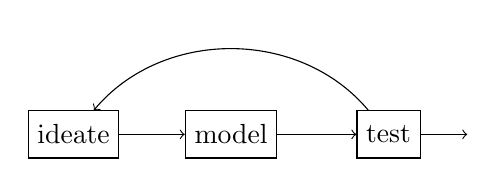
\begin{tikzpicture}[
    every node/.append style={draw, minimum height=0.6cm}]
    \node (ideate_name) at (0,0) {ideate};
    \node (model_name) at (2,0) {model};
    \node (test_name) at (4,0) {test};

    \path[->]
        (ideate_name) edge (model_name)
        (model_name) edge (test_name)
        (test_name) edge[bend right=50] (ideate_name)
        (test_name) edge (5,0);
\end{tikzpicture}




\begin{tikzpicture}[
    every node/.append style={draw, minimum size=0.5cm}]
    \node[ultra thin] at (0,0) {};
    \node[very thin] at (1,0) {};
    \node[thin] at (2,0) {};
    \node[semithick] at (3,0) {};
    \node[thick] at (4,0) {};
    \node[very thick] at (5,0) {};
    \node[ultra thick] at (6,0) {};
\end{tikzpicture}




\begin{tikzpicture}[
    every node/.append style={draw, minimum size=0.5cm}]
    \node at (0,0) {};
    \node[dashed] at (1,0) {};
    \node[dashdotted] at (2,0) {};
    \node[dotted] at (3,0) {};
    \node[loosely dotted] at (5,0) {};
    \node[densely dotted] at (6,0) {};
\end{tikzpicture}



\begin{tikzpicture}[
    every node/.append style={minimum size=0.5cm}]
    \node[draw=blue] at (0,0) {};
    \node[fill=blue] at (1,0) {};
    \node[fill=blue!50!cyan] at (2,0) {};
    \node[fill=cyan] at (3,0) {};
    \node[fill=cyan!50] at (4,0) {};
    \node[draw=cyan,text=cyan] at (5,0) {hi};
\end{tikzpicture}




\begin{tikzpicture}[
    every node/.append style={draw}]
    \node at (0,0) {default};
    \node[rectangle] at (2,0) {rectangle};
    \node[circle] at (4,0) {circle};
\end{tikzpicture}


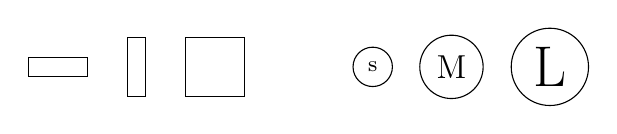
\begin{tikzpicture}[
    every node/.append style={draw}]
    \node[minimum width=0.75cm] at (0,0) {};
    \node[minimum height=0.75cm] at (1,0) {};
    \node[minimum size=0.75cm] at (2,0) {};
    \node[circle] at (4,0) {\footnotesize s};
    \node[circle] at (5,0) {\large M};
    \node[circle] at (6.25,0) {\huge L};
\end{tikzpicture}




\begin{tikzpicture}[
    every node/.append style={draw,thick,text=cyan}]
    \node[inner sep=-2pt] at (0,0) {Hi};
    \node[inner sep=0pt] at (1,0) {Hi};
    \node at (2,0) {Hi};
    \node[inner sep=8pt] at (3.25,0) {Hi};

    \node[inner xsep=8pt] at (5.5,0) {Hi};
    \node[inner ysep=8pt] at (7,0) {Hi};
\end{tikzpicture}



\begin{tikzpicture}
    \path[ultra thin] (0,2) edge (0,2.5);
    \path[very thin] (1,2) edge (1,2.5);
    \path[thin] (2,2) edge (2,2.5);
    \path[semithick] (3,2) edge (3,2.5);
    \path[thick] (4,2) edge (4,2.5);
    \path[very thick] (5,2) edge (5,2.5);
    \path[ultra thick] (6,2) edge (6,2.5);

    \path (0,1) edge (0,1.5);
    \path[dashed] (1,1) edge (1,1.5);
    \path[dashdotted] (2,1) edge (2,1.5);
    \path[dotted] (3,1) edge (3,1.5);
    \path[loosely dotted] (5,1) edge (5,1.5);
    \path[densely dotted] (6,1) edge (6,1.5);

    \path (0,0) edge (0,0.5);
    \path[gray] (1,0) edge (1,0.5);
    \path[blue] (2,0) edge (2,0.5);
    \path[violet] (3,0) edge (3,0.5);
    \path[magenta] (4,0) edge (4,0.5);
    \path[purple] (5,0) edge (5,0.5);
    \path[red] (6,0) edge (6,0.5);
\end{tikzpicture}


\begin{tikzpicture}
    \path (0,1) edge (0,1.5);
    \path[->] (1,1) edge (1,1.5);
    \path[<-] (2,1) edge (2,1.5);
    \path[<->] (3,1) edge (3,1.5);
    \path[<<->>] (4,1) edge (4,1.5);
    \path[<<<->>>] (5,1) edge (5,1.5);
    \path[-to] (6,1) edge (6,1.5);

    \path[stealth-stealth] (0,0) edge (0,0.5);
    \path[stealth reversed-stealth reversed] (1,0) edge (1,0.5);
    \path[to-to] (2,0) edge (2,0.5);
    \path[to reversed-to reversed] (3,0) edge (3,0.5);
    \path[latex-latex] (4,0) edge (4,0.5);
    \path[latex reversed-latex reversed] (5,0) edge (5,0.5);
    \path[|-|] (6,0) edge (6,0.5);
\end{tikzpicture}


\begin{tikzpicture}
    \node[draw] (x) {$X$};
    \node[draw,right=1cm of x] (y) {$Y$};
    \path[->]
        (x) edge[bend left=30] node[pos=0.5,above] {$G$} (y)
        (y) edge[bend left=30] node[pos=0.5,below] {$F$} (x);
\end{tikzpicture}


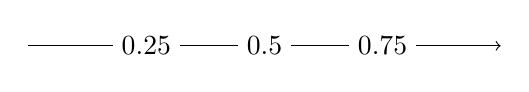
\begin{tikzpicture}[every node/.append style={fill=white}]
    \path[->] (0,0) edge
        node[pos=0.25] {0.25}
        node[pos=0.5] {0.5}
        node[pos=0.75] {0.75}
    (6,0);
\end{tikzpicture}


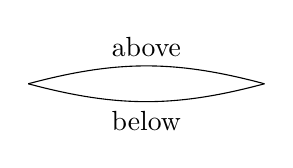
\begin{tikzpicture}
    \path (0,0)
        edge[bend left=15] node[pos=0.5,above] {above} (3,0)
        edge[bend right=15] node[pos=0.5,below] {below} (3,0);
\end{tikzpicture}


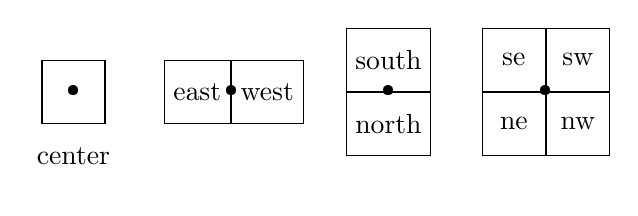
\begin{tikzpicture}[every node/.append style={draw, minimum size=0.8cm}]
    \node[draw=none] at (0,0) {\textbullet};
    \node[anchor=center, label=below:{center}] at (0,0) {};
    \node at (0,0) {};

    \node[draw=none] at (2,0) {\textbullet};
    \node[anchor=west] at (2,0) {west};
    \node[anchor=east] at (2,0) {east};

    \node[draw=none] at (4,0) {\textbullet};
    \node[anchor=north] at (4,0) {north};
    \node[anchor=south] at (4,0) {south};

    \node[draw=none] at (6,0) {\textbullet};
    \node[anchor=north west] at (6,0) {nw};
    \node[anchor=north east] at (6,0) {ne};
    \node[anchor=south east] at (6,0) {se};
    \node[anchor=south west] at (6,0) {sw};
\end{tikzpicture}


\begin{tikzpicture}
    \draw[help lines] (-2,-2) grid (2,2);
    \node (0) {origin};
    \node[right=of 0] {right};
    \node[below right=of 0] {below right};
    \node[below=of 0] {below};
    \node[below left=of 0] {below left};
    \node[left=of 0] {left};
    \node[above left=of 0] {above left};
    \node[above=of 0] {above};
    \node[above right=of 0] {above right};
\end{tikzpicture}


\begin{tikzpicture}
    \node[label=left:left] at (0,0) {\textbullet};
    \node[label=above:above] at (2,0) {\textbullet};
    \node[label=below:below] at (4,0) {\textbullet};
    \node[label=right:right] at (6,0) {\textbullet};
\end{tikzpicture}


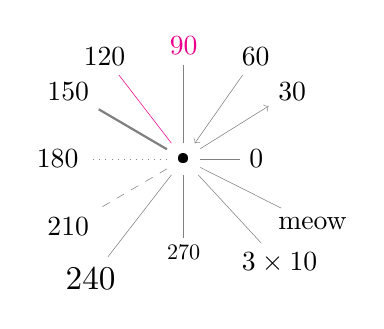
\begin{tikzpicture}[pin distance=10mm]
    \node[pin={[pin distance=5mm]0:0},
          pin={[pin edge={->}]30:30},
          pin={[pin edge={<-}]60:60},
          pin={[magenta]90:90},
          pin={[pin edge={magenta}]120:120},
          pin={[pin edge={thick}]150:150},
          pin={[pin edge={dotted}]180:180},
          pin={[pin edge={dashed}]210:210},
          pin={[scale=1.2]240:240},
          pin={[scale=0.8]270:270},
          pin={300:$3\times10$},
          pin={330:meow}]
    at (11,-2) {\textbullet};
\end{tikzpicture}


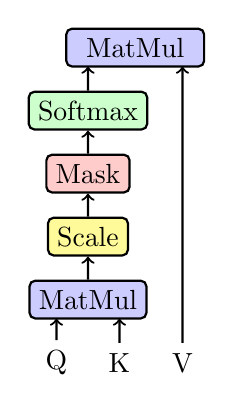
\begin{tikzpicture}[scale=0.8,
    every node/.append style={thick,rounded corners=2pt}]
    \node (q) at (.5,0) {Q};
    \node (k) at (1.5,0) {K};
    \node (v) at (2.5,0) {V};

    \node[draw,fill=blue!20] (matmul1) at (1,1) {MatMul};
    \node[draw,fill=yellow!40] (scale) at (1,2) {Scale};
    \node[draw,fill=red!20] (mask) at (1,3) {Mask};
    \node[draw,fill=green!20] (softmax) at (1,4) {Softmax};
    \node[draw, fill=blue!20, minimum width=1.75cm] (matmul2) at (1.75,5) {MatMul};

    \path[->,thick]
        (matmul1) edge (scale)
        (scale) edge (mask)
        (mask) edge (softmax)
        (q) edge (.5,.7)
        (k) edge (1.5,.7)
        (v) edge (2.5,4.7)
        (softmax) edge (1,4.7);
\end{tikzpicture}



